\section{Stefan-Boltzmann Law}

\makelabheader


\paragraph{Introduction.}
Stars (and other astronomical objects) emit a lot of their energy
in the form of \textit{thermal radiation}. To understand how these objects
work, we need to know how much energy they emit. In this lab, you'll
examine the relationship between the amount of \textit{power} (that is,
energy per time) emitted
by an object and the object's \textit{temperature}.

The apparatus for this experiment consists of a lamp and a radiation sensor.
The lamp will be hooked up to a power supply, and the radiation sensor
is attached to a meter that indicates the intensity of light
striking it.

\centerline{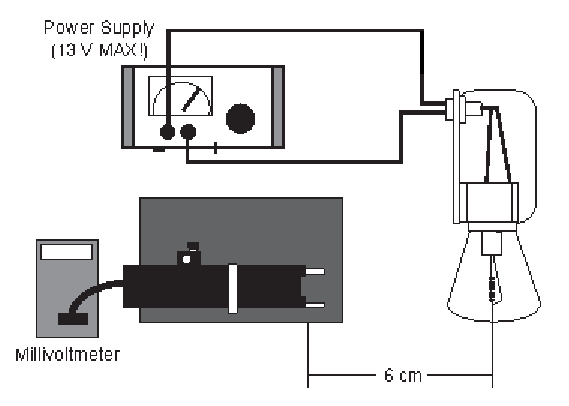
\includegraphics{stefan/stefan1.pdf}}

By changing the voltage being applied to the lamp, we can change its
temperature. The radiation sensor then tells us how much power is being
emitted at any given temperature.

We're going to want to know how the power depends on the temperature of the
lamp filament. We can't conveniently attach a thermometer to the filament,
so we have to get the temperature another way, namely by measuring
the filament's \textit{resistance}, which depends on the temperature
in a known way. Here's how this works.

Suppose we apply a certain number of volts $V$ to the lamp. That voltage
will cause electric current to flow through the lamp. We'll measure
the amount of current, which is traditionally called $I$ (for some reason). 
The resistance is the ratio of these two:
$$
R = {\frac{V} I}.
$$
The value of $R$ increases in a known way as the temperature goes
up, so by keeping track of $R$ we'll be able to keep track of the
temperature.

\pagebreak[3]

\paragraph{Gathering the data.}
The first thing you'll need to know is the resistance $R$ of the filament
when it's at room temperature. We'll do this by applying a small voltage
to the lamp, and recording the amount of current that flows. If we keep
the voltage small, we can assume that the lamp won't heat up very much,
so we can use these values to figure out the resistance at 
room temperature.

Connect the lamp to the power supply as shown in the diagram.
Turn the voltage knob all the way to zero (counterclockwise), and turn
the current knob up (clockwise). Now turn on the power supply.
The voltage display on the power supply should read zero. Turn up the voltage
knob gradually until it reads about 0.5 volts.

At this point, the power supply is supplying a small amount of energy to push
a small amount of current through the lamp. It's not enough to heat up
the filament significantly or to make the lamp glow. 
Record the voltage ($V$) and current ($I$) readings on the power supply here. The voltage 
should be 0.5 V, and the current is some number of ``amperes'' (A).

\answerspace{0.5in}
$$
V=\qquad\qquad\qquad
I = \qquad\qquad\qquad\ 
$$
\answerspace{0.5in}
Use the rule $R={\frac{V} I}$ to determine the resistance. 
The unit of resistance is called the ``ohm'' and is written $\Omega$.

\answerspace{0.5in}
$$
R_{300\,{\rm K}}=
$$
\answerspace{0.5in}

You might wonder why we call it by the strange name $R_{300\,{\rm K}}$.
The reason is that this is the value of the resistance at room temperature, 
which corresponds to a 
temperature of about 300 kelvin. 

Now that you have this, you can start taking measurements when the lamp
is actually glowing. First, make sure that the lamp is at the same height
as the radiation detector, and the distance between the two is about 6 cm.
The exact distance doesn't matter, but it's important that it not 
change once you start measuring. Make sure that the detector is facing
directly toward the lamp and there are no other bright light sources
in its path. The radiation sensor should be hooked up to the
voltmeter's inputs labeled COMMON and V/$\Omega$, and it should 
be set to read DC voltage. That setting on the meter's dial will
probably look like a V with straight lines (not a wavy line) 
next to it or above it.
Check with me to see if you've got everything wired up correctly.

Once you're ready, turn up the voltage dial gradually until it reads 2 volts.
You should see the lamp glowing faintly.

In the data table at the end of this lab, record the voltage $V$ (which is 2 V),
the current $I$ from the display on the power supply,
and the reading on the voltmeter
attached to the radiation sensor. The last number is a measure
of the power being radiated by the lamp, so we'll call it $P$. 
Record these values
in the first row of the table on the last page of this lab. (Leave
the other columns in this table blank for now.)

Once you've done this, repeat for voltages of 4, 6, 8, 10, 12 V.

You should expose the radiation sensor to the lamp light only briefly
when you're making each power measurement. In between measurements, place 
sheets of insulating foam between the lamp and the sensor, with the silvered
surface facing the lamp, so that the temperature of the radiation sensor
stays fairly constant.


\paragraph{Analyzing the data.}
You'll need to determine the temperature of the filament during each of these
measurements, by filling in the remaining columns in the data table. Here's
how. 

First, find the value of the resistance for each row, using the rule $R={\frac{V} 
I}$. 

The temperature is determined by how this resistance compares with its
value at room temperature, so compute the ratio ${\frac{R} R_{300\,{\rm K}}}$
for each row.

The graph near the end of the lab 
shows how this ratio is related to temperature.
For each row in the table, use the graph to determine the value of 
temperature corresponding to the resistance ratio you've determined.
(Read across the graph at the height corresponding to the ratio.
When you hit the curve, go straight down to get the temperature.)

Once you've done this, the data table should be filled in.
Now we want to graph it, using \textit{excel}. Appendix B of your
lab manual contains some information about making graphs in \textit{excel}.
Create an \textit{excel} data table with two columns, $T$ and $P$. (Put
$T$ on the left.) Following the instructions in Appendix B.2, make
a graph showing how $P$ depends on $T$. 

You should find that the power goes up as the temperature goes up.

We want to see what sort of mathematical relationship matches this graph. 
Try adding a ``trendline'' to the chart, following the instructions
in Appendix B.3.
This shows the straight line
that matches the data as well as possible. Does a straight line look
like a good fit to this set of data?

\answerspace{1in}

Double-click on the trendline to get various options to customize it.
You should see various options such as ``Exponential,'' ``Linear,'' etc.
These replace the straight-line relationship with various other 
mathematical relationships. You can try all of these out to see
which ones look like a good match to the data.

In the end, we'll be most interested in the one called ``Power.'' Select
this trendline option, and also check the box that says ``Display
equation on chart.'' What this does is to find the best-fitting mathematical
relationship of the form $y=\mbox{(something)}\times x^{\mbox{(something)}}$
between the two quantities in the graph. In our case, $x$ and $y$
are $T$ and $P$ respectively.

According to \textit{excel}, what is the best-fitting value
of the exponent (the power of $x$) in this relationship?

\answerspace{1in}

What do we expect this exponent to be, according to the Stefan-Boltzmann
Law? (If you don't remember this from your reading, you can look it up.)

\answerspace{1in}

Does your data agree reasonably well with the Stefan-Boltzmann Law?


\centerline{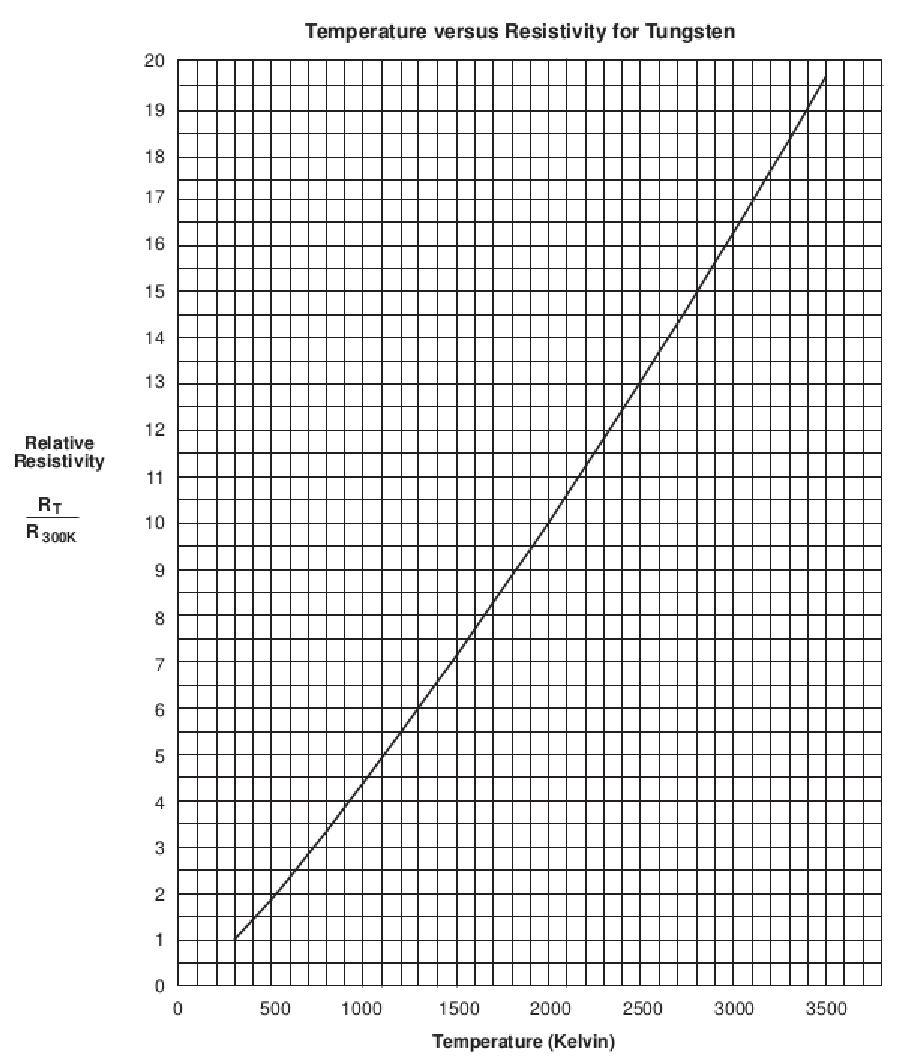
\includegraphics{stefan/stefan2.pdf}}





\begin{center}
\begin{tabular}{|p{0.8in}|p{0.8in}|p{0.8in}|p{0.8in}|p{0.8in}|p{0.8in}|} \hline
$V$ (volts) & $I$ (amps) & $P$ (mV) & $R$ ($\Omega$) & $R/R_{300
\,{\rm K}}$\ & $T$ (K) \\ \hline
\ & \ & \ & \ & \ & \ \\
\ & \ & \ & \ & \ & \ \\
\ & \ & \ & \ & \ & \ \\
\ & \ & \ & \ & \ & \ \\ \hline
\ & \ & \ & \ & \ & \ \\
\ & \ & \ & \ & \ & \ \\
\ & \ & \ & \ & \ & \ \\
\ & \ & \ & \ & \ & \ \\ \hline
\ & \ & \ & \ & \ & \ \\
\ & \ & \ & \ & \ & \ \\
\ & \ & \ & \ & \ & \ \\
\ & \ & \ & \ & \ & \ \\ \hline
\ & \ & \ & \ & \ & \ \\
\ & \ & \ & \ & \ & \ \\
\ & \ & \ & \ & \ & \ \\
\ & \ & \ & \ & \ & \ \\ \hline
\ & \ & \ & \ & \ & \ \\
\ & \ & \ & \ & \ & \ \\
\ & \ & \ & \ & \ & \ \\
\ & \ & \ & \ & \ & \ \\ \hline
\ & \ & \ & \ & \ & \ \\
\ & \ & \ & \ & \ & \ \\
\ & \ & \ & \ & \ & \ \\
\ & \ & \ & \ & \ & \ \\ \hline
\end{tabular}
\end{center}
